\section{Simulation}
\subsection{Initial work in Python}
Initially, work undertaken by the simulation group consisted of finding suitable mechanical descriptions of the droplet's motion, and implementing those in code. A simplified model was taken from \cite{brady2014bouncing}, where the droplet was treated as stationary in the x-y plane and moving in z according to (\ref{equ:basicHeight}). Here, $h_0$ is the maximum height of the drop, $\omega_0$ is the driving frequency of the system, r is the displacement of the drop from the centre in polar co-ordinates and c is the speed of the wave. $J_0$ is a Bessel function of the first kind. With $\omega_0$, r and c set arbitrarily to 1, wave motion was demonstrated using an animation framework from \cite{waveanimation}. The results of this are shown in Figure \ref{fig:basicAnimation}. Unfortunately, the Python language used to generate this proved too slow to be usable as a live demonstration, so any simulations generated using this method would need to be exported to a movie file and played back later. This was deemed an unacceptable solution, and so Java was chosen as a more efficient language to use in future.

\begin{equation}
    h = -h_0 \cos{(\omega_0 t)} J_0 (\omega_0 r/c)
    \label{equ:basicHeight}
\end{equation}

\begin{figure}[h]
    \begin{subfigure}{0.5\textwidth}
        \centering
        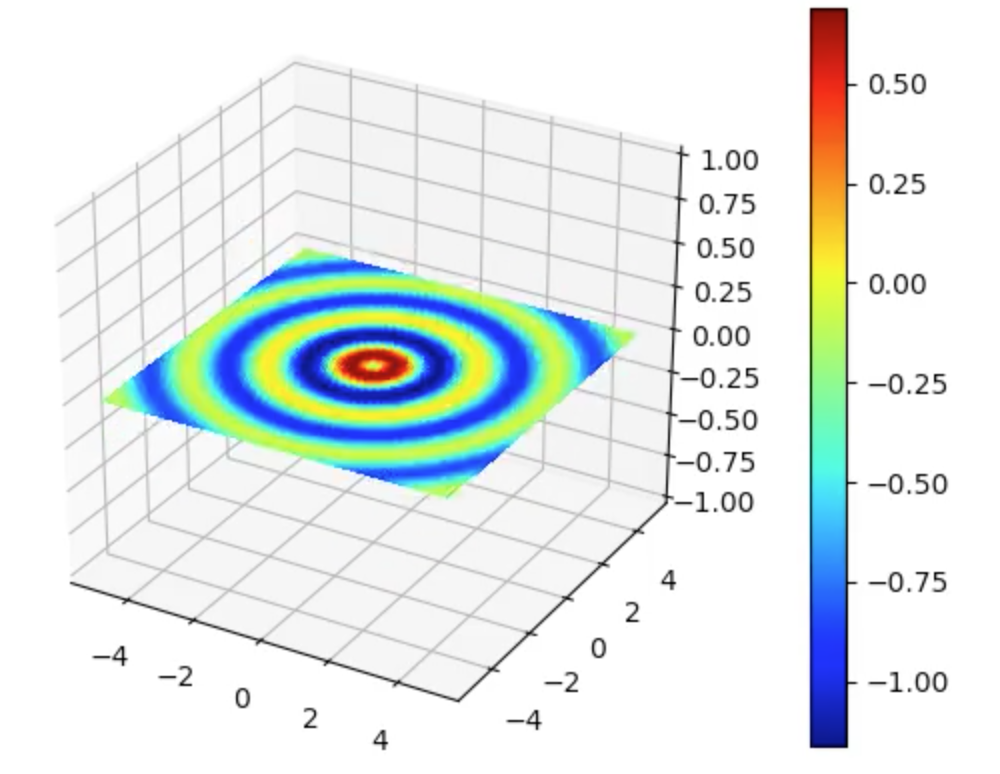
\includegraphics[width=\linewidth]{simulation/basich0.png}
        \caption{Wave motion at $h=0$}
    \end{subfigure}
    \begin{subfigure}{0.5\textwidth}
        \centering
        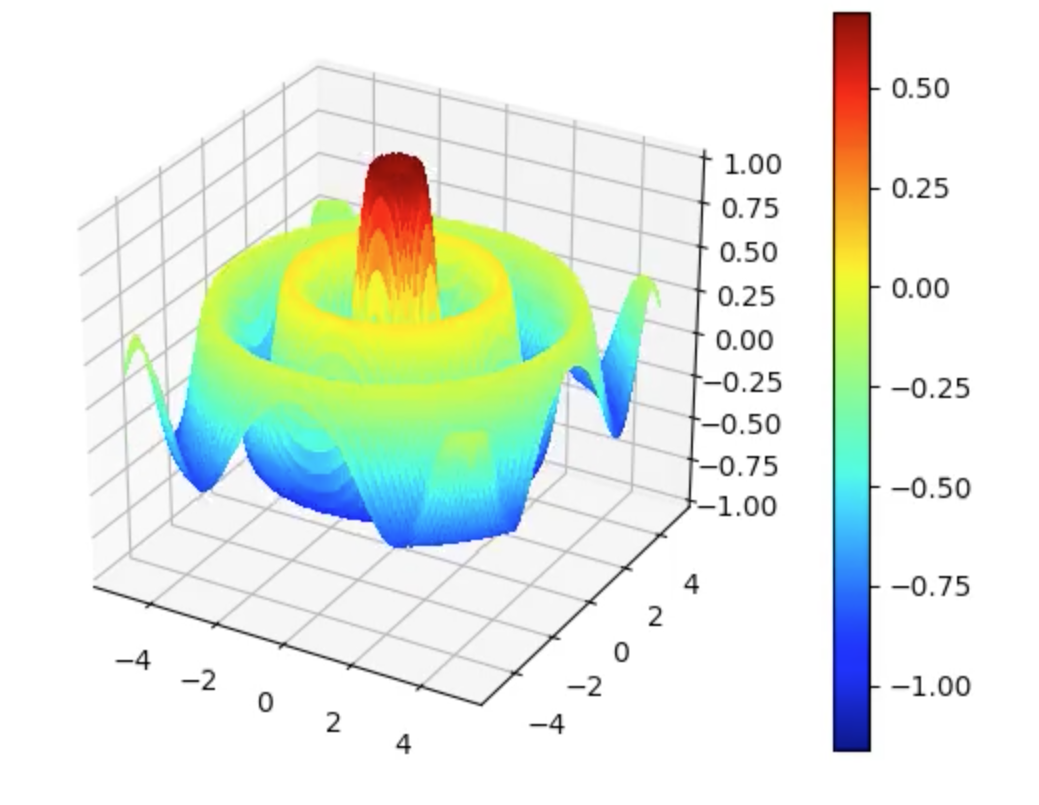
\includegraphics[width=\linewidth]{simulation/basichmax.png}
        \caption{Wave motion at $h=h_0$}
    \end{subfigure}
\caption{Simulation output generated with Python and Matplotlib. (a) represents the initial state of the wavefield, while (b) represents the state of the wave-field when the "droplet" at the centre is at its maximum height}
\label{fig:basicAnimation}
\end{figure}

\subsection{Constructing a GUI in Java}
Initial versions of the Java simulation aimed to construct a pixel grid which could be used to represent a wavefield. Objects representing a given data point and a "frame" of these data points were constructed, and populated with amplitudes using (\ref{equ:basicHeight}). These amplitudes were then displayed in 2D by assigning them to an opacity scale, with 100\% opacity representing the maximum possible height and 100\% transparency representing the minimum possible height. For a 40,000 pixel frame running over 10 seconds, this process took approximately 9 seconds, but the animation process after this ran in real time. Figure \ref{fig:javaBasicHeight} shows a still image of this GUI taken when the "droplet" was at a minimum height of $-h_0$. This animation was a success, but at higher resolutions, latency when drawing the pixels to the screen caused it to lag, suggesting a need to either run multiple drawing tasks in parallel, or to display the droplet motion in an alternative way.

\begin{figure}
    \centering
    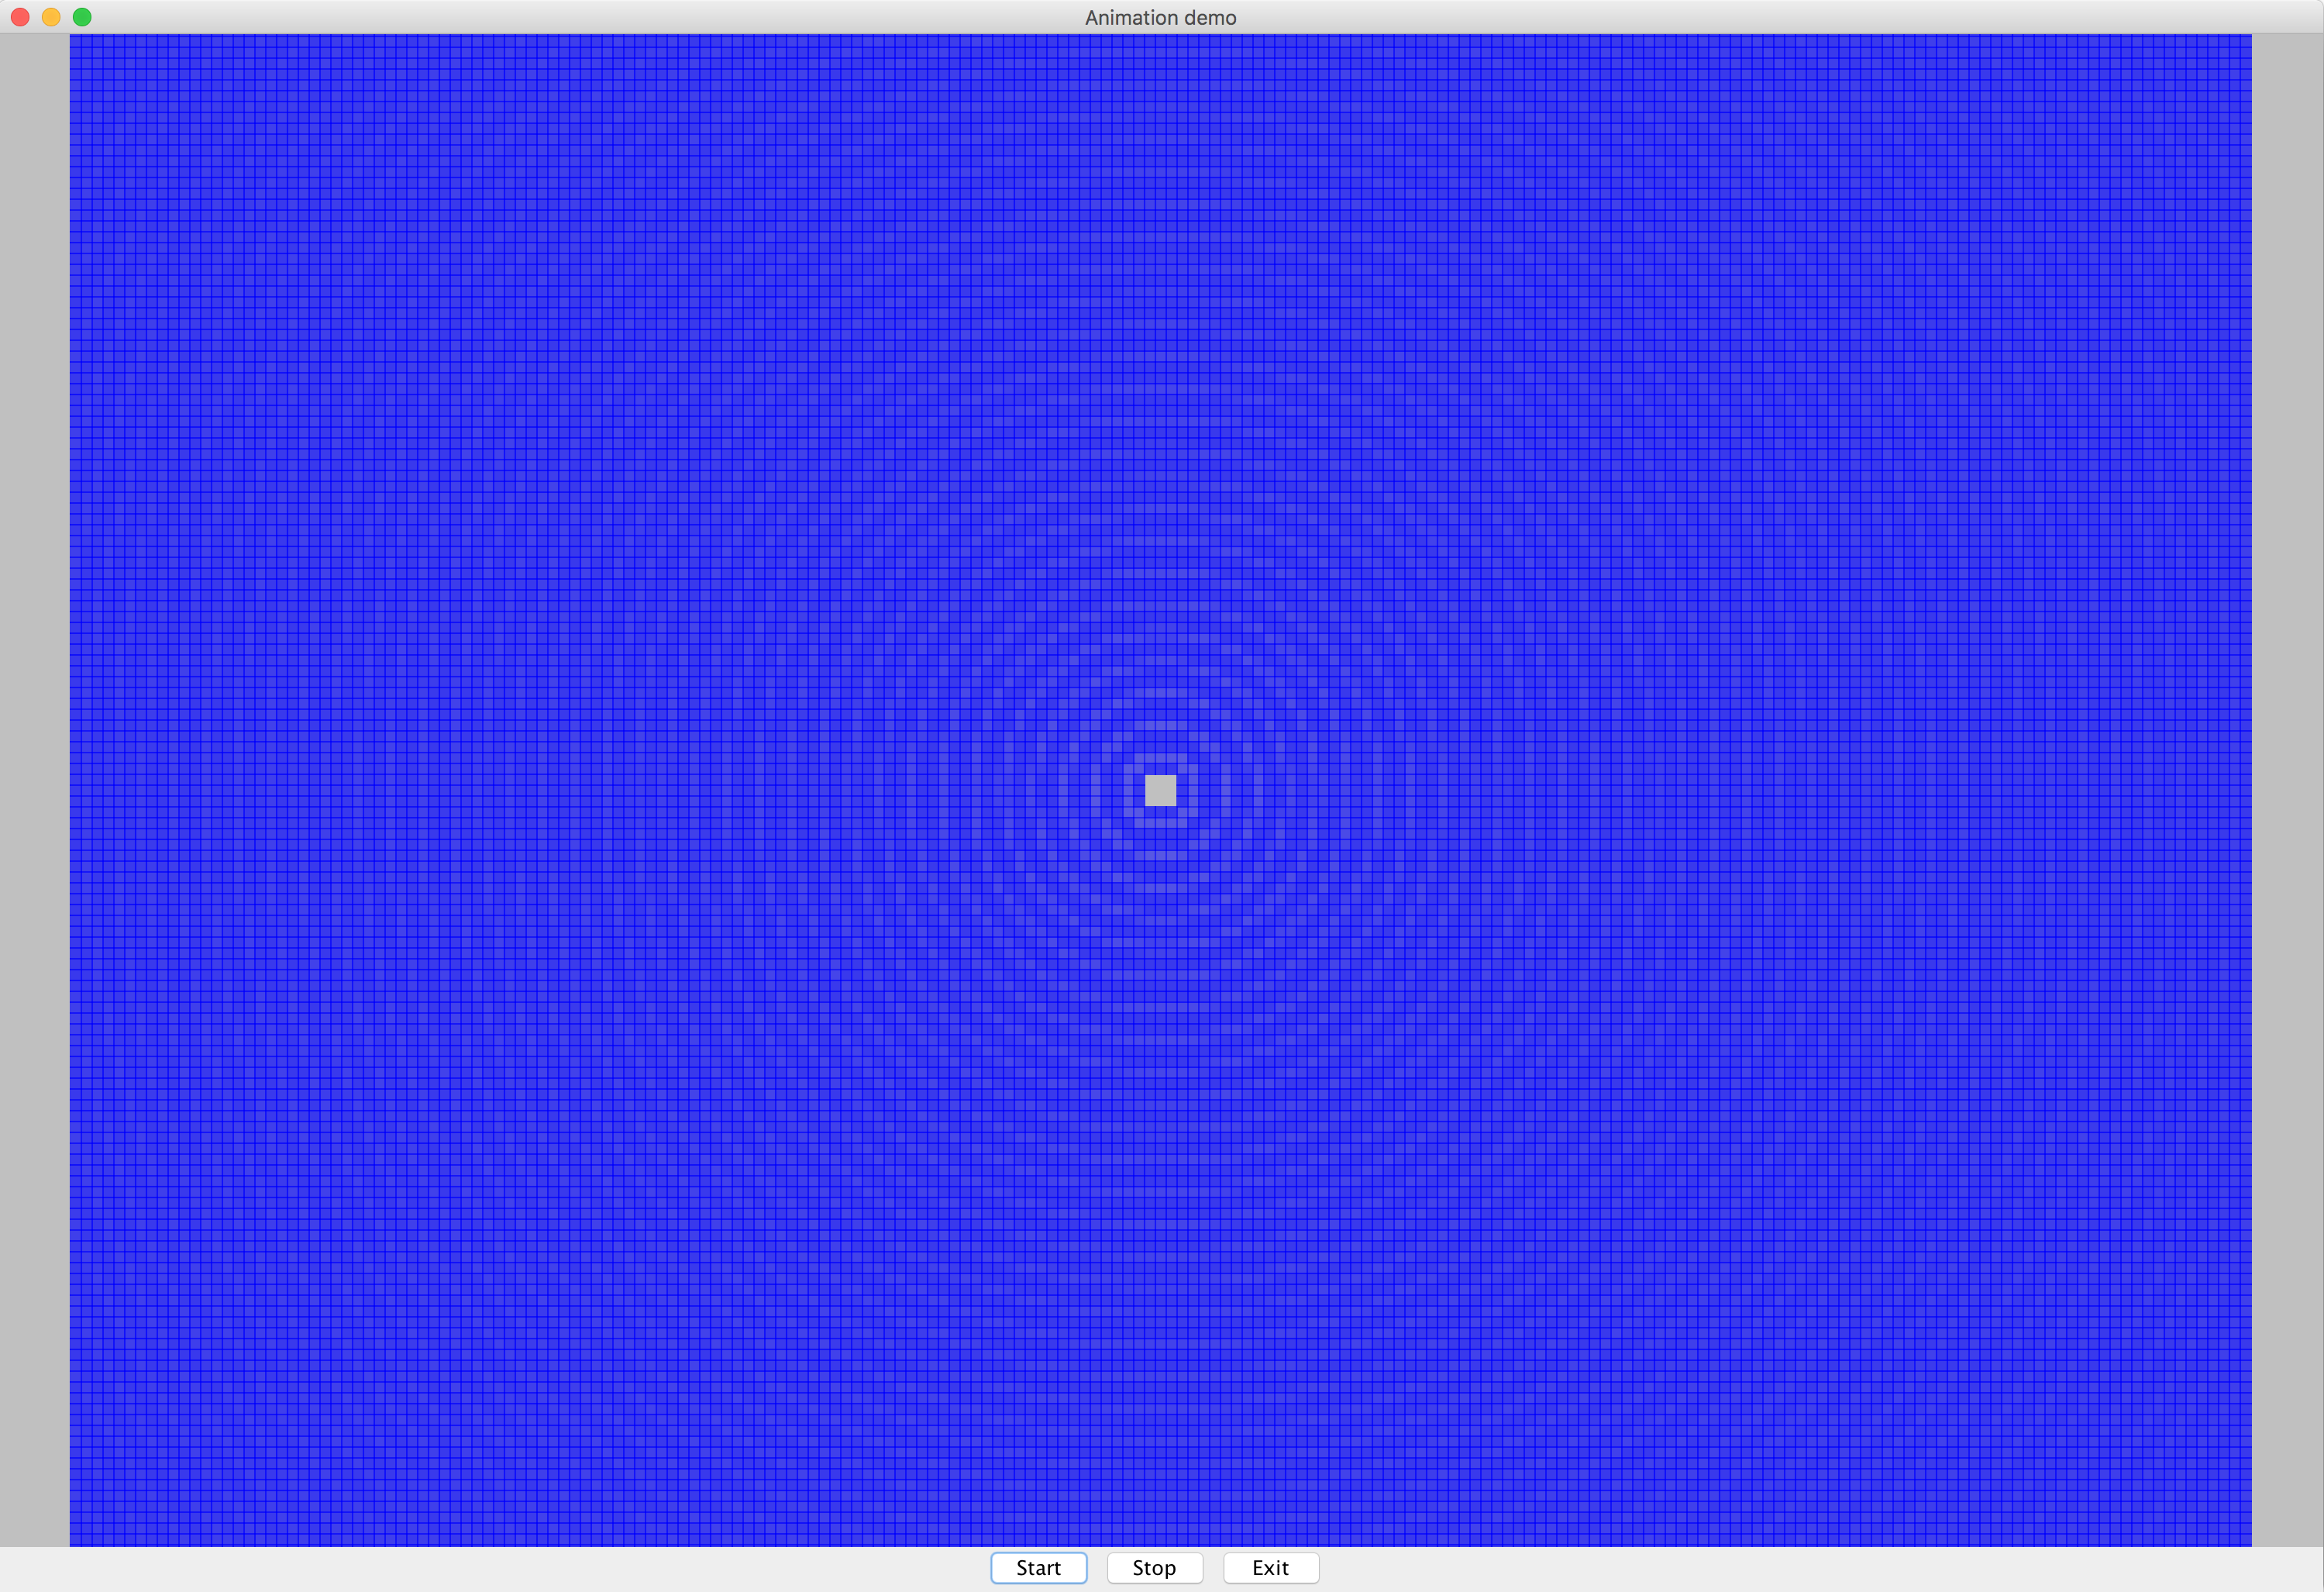
\includegraphics[width=\textwidth]{simulation/javaMaxHeight.png}
    \caption{A basic Java GUI, here showing the droplet at its minimum height of $-h_0$}
    \label{fig:javaBasicHeight}
\end{figure}

\subsection{Probabilistic Prediction of Position}
Having demonstrated the possibility of displaying wave-functions in Java, displaying an object representing a droplet was the next task. Here, the assumption was that the wave (described by Equation \ref{equ:probWaveEqn}) represented a probability density function. Therefore, for a given (and ideally infinitesimal) pixel n of area dA, the probability $P_n$ of finding the particle at pixel $n$ was calculated from that function. The height ($z_n$) of each pixel within that section was calculated, with ${P_n}/{z_n}$ representing the probability of the particle being at that pixel. The sum of probabilities for this section, $Z=\sum_n{P_n}$, defined the normalisation value of the thread. A random number generator then generated a number R such that $0\leq R \leq 1$, which was multiplied by $Z$ to give a relative random number. The program then looped back over all the pixels in the section, and repeatedly subtracts $P_n$ from $RZ$ until $RZ<0$. The first pixel where this condition is satisfied is determined to be the location of the droplet. This process could then be multi-threaded to improve computational efficiency.

The application of this to our project was that once the droplet is found at a given pixel, the distance between that pixel and the next pixel representing the location of the droplet is used to calculate the velocity v of the particle, assuming the droplet moves to the new pixel in the space of one period $T=1/f$. The wave-function was updated with the new velocity, once a Lorentz transform was accounted for. This whole process is repeated to find the trajectory of the pixel.

\begin{figure}
\centering
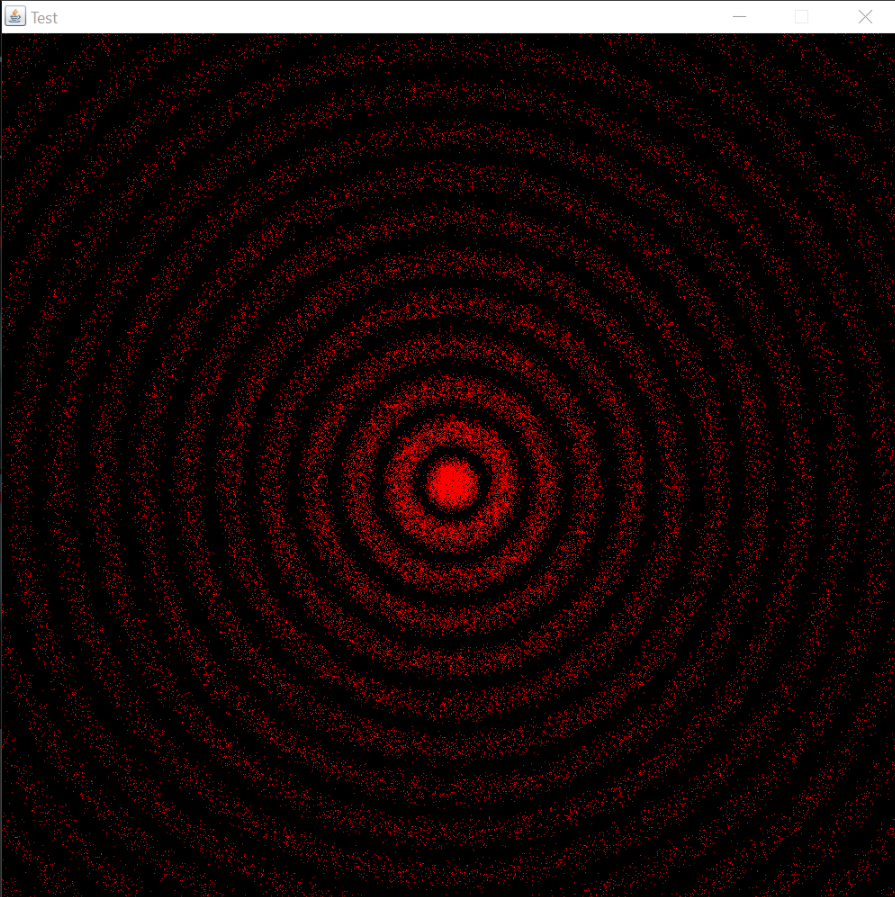
\includegraphics[width=\textwidth]{simulation/probabiltyPosition.png}
\caption{Results of the probabilistic prediction of the droplet position, where each dot represents the droplet being present at this point}
\label{fig:probabilisticPrediction}
\end{figure}

\begin{equation}
    NEED TO COMPLETE
    \label{equ:probWaveEqn}
\end{equation}

Although this process was successful, all it ended up proving was that a random position generator works. It does not accurately simulate the position of droplets created in our experiment. Therefore, we proceeded to calculate the equations of motion and the wave-function of the droplet at each point.



$$h = -h_0 \cos{(\omega_0 t - \frac{\gamma^2\omega_0 v}{c^2} \Delta x)}J_0(\omega_0 r''/c)$$

$$ h = -h_0 J_0(\omega_0 r''/c)$$

$$\gamma = (1-\frac{v^2}{c^2})^{-{\frac{1}{2}}}$$

$$\Delta x = x - vt$$

$$r'' = \sqrt{\gamma^4(x-vt)^2 + (\gamma y)^2}$$

$$H = \sum_i h_i D(i)$$



